\section{Проектирование асинхронного фреймворка}

При проектировании асинхронной модели фреймворка была существенно изменена архитектура синхронного ядра. Так же при проектировании были учтены выявленные архитектурные ошибки в синхронных версиях. Данная реализация системы подразумевает использование высокоскоростных алгоритмов десериализации. При тестировании данной системы исползовалась библиотека Google Flat Buffers, но данная реализация позволяет применять любой алгоритм сериализации/десериализации с использованием бинарного буфера памяти.

Отличие асинхронной версии от синхронной в первую очередь заключается в том, что система сама уведомляет о всех изменениях: модули регистрируют функции обратного вызова для получения требуемой информации о состоянии системы при ее изменениях.

\begin{figure}[h]
    \centering{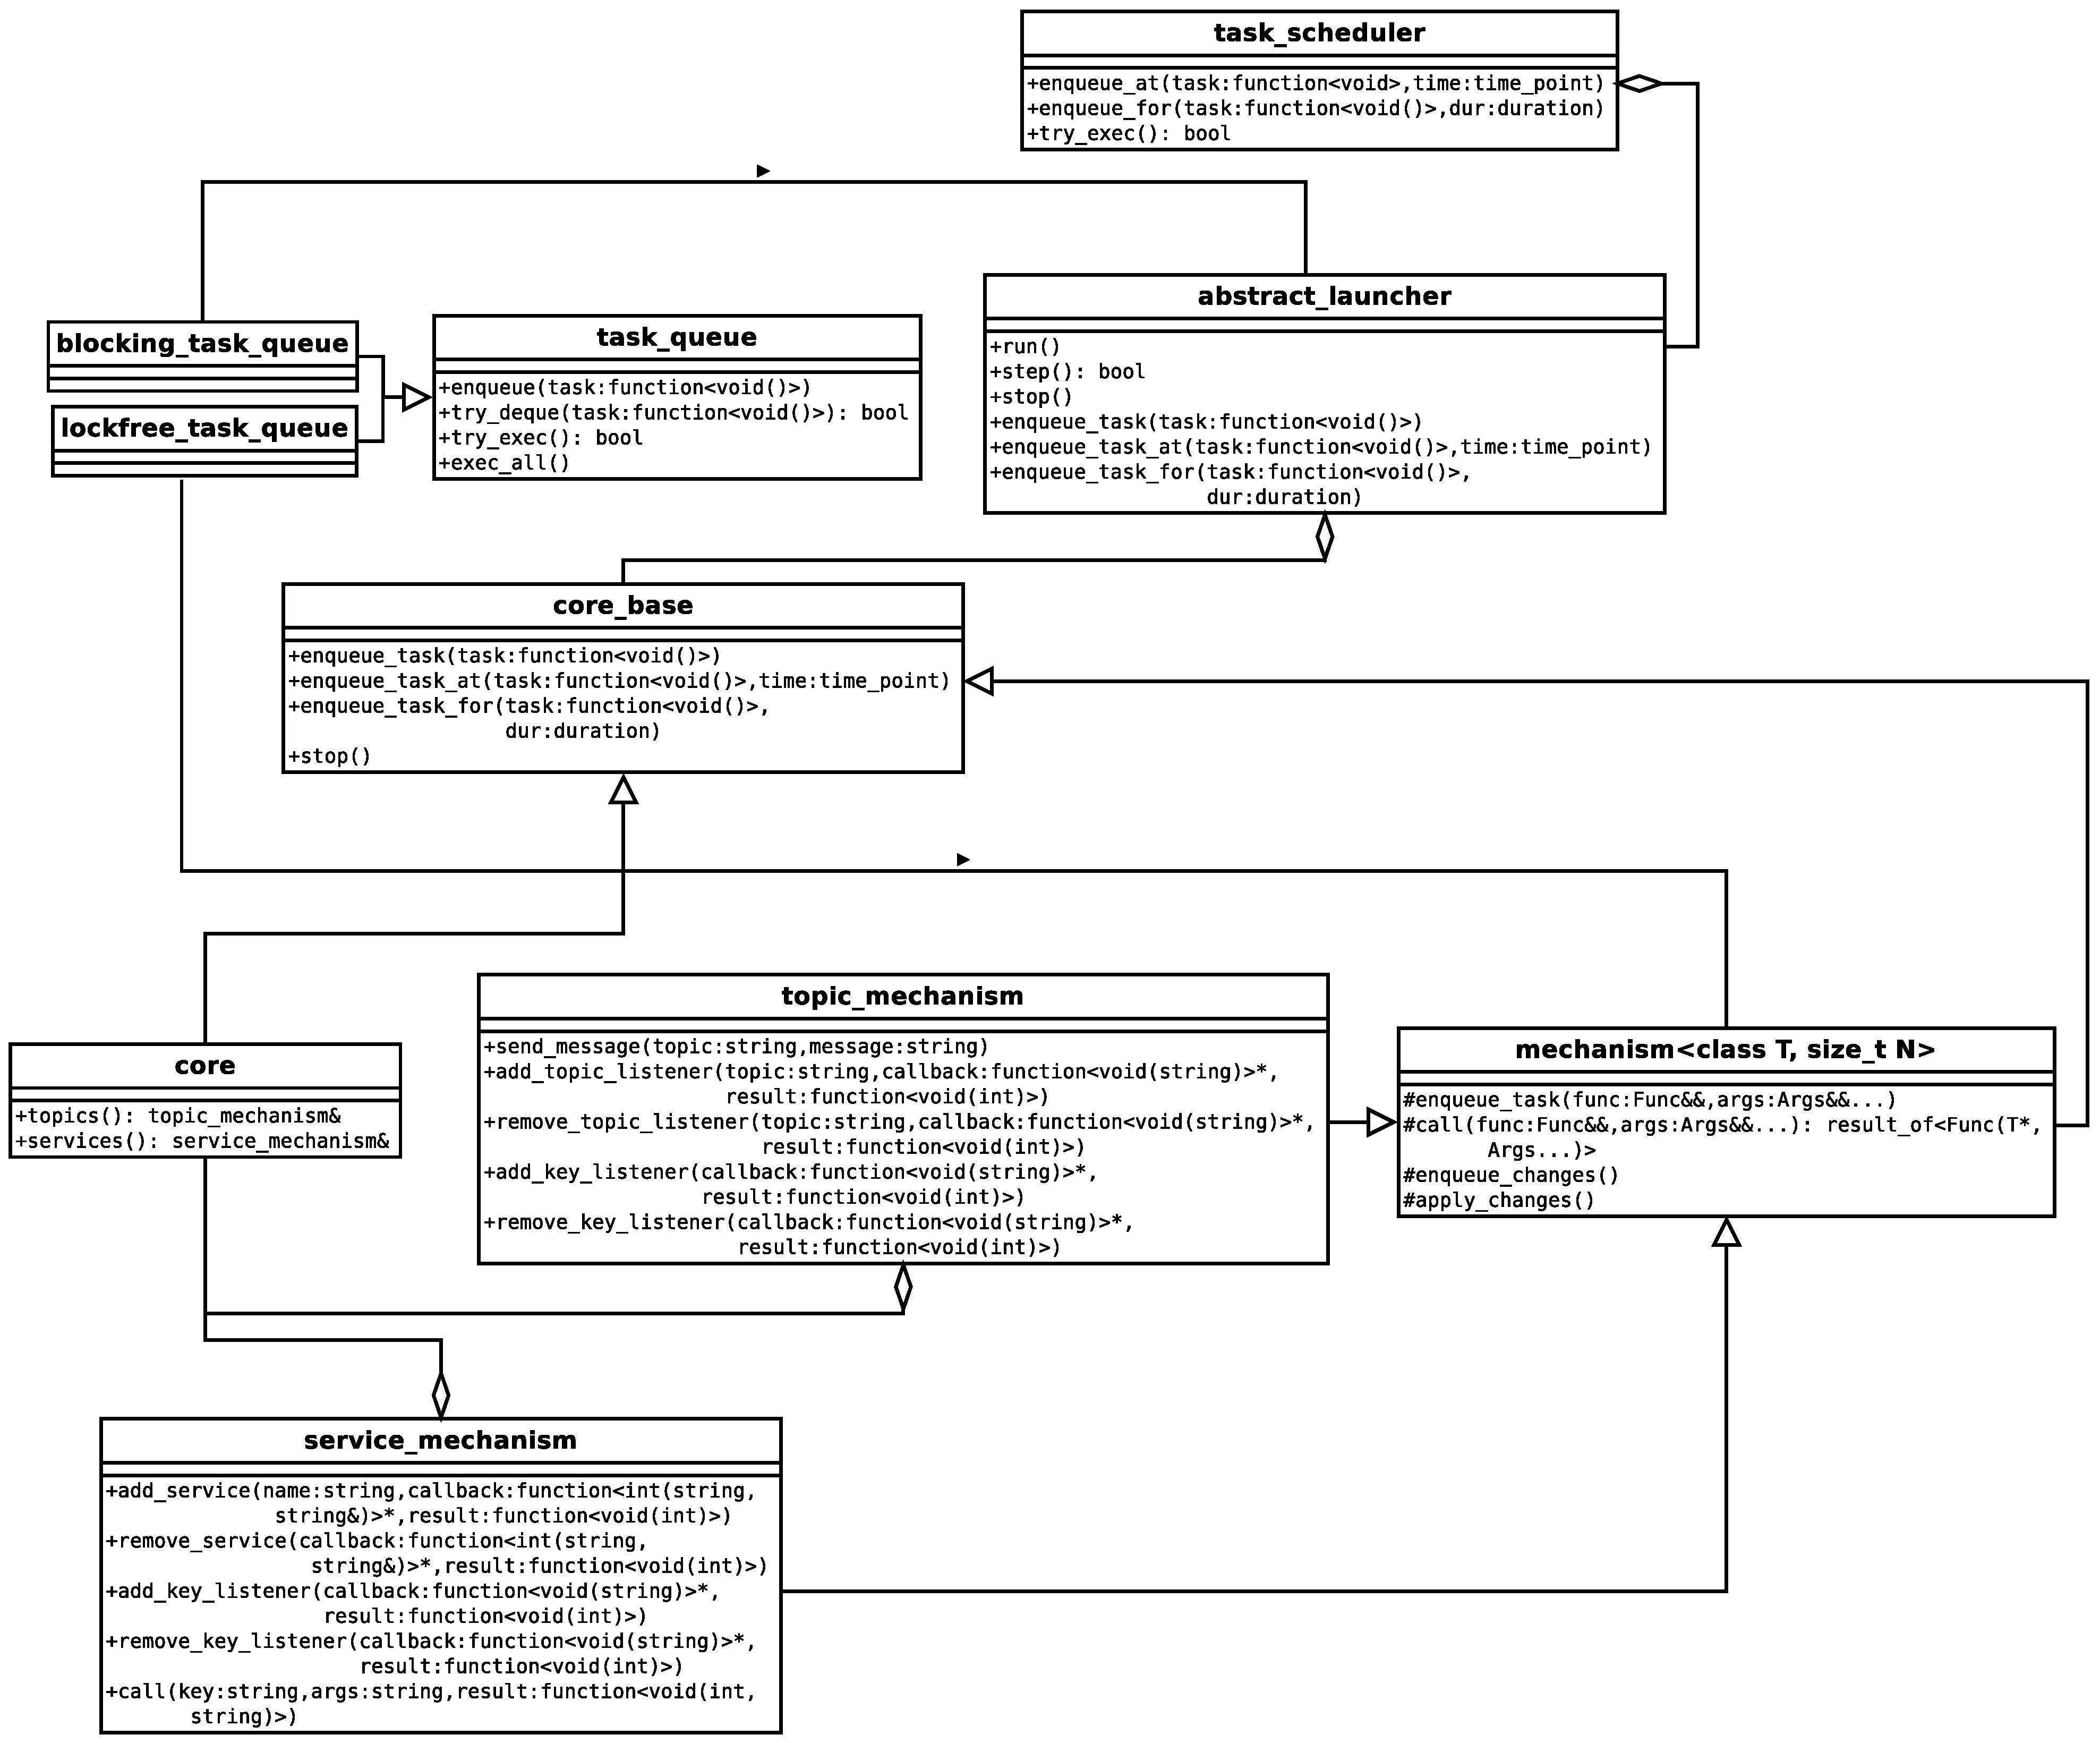
\includegraphics[width=1\linewidth]{2_3_1_async}}
    \caption{Диаграмма классов асинхронной версии фреймворка}
    \label{im:2_3_1_async}
\end{figure}

\textit{abstract\_launcher} --- задачи данного класса схожи с аналогичным классом из синхронной версии фреймворка: класс определяет порядок и способ исполнения задач. Синхронная версия расширенна функциями планировщика для выполнения задачи в определенный момент времени или спустя заданный промежуток времени. Обращения к этому классу могут происходить напрямую из разных потоков и поэтому реализация должна учитывать данный фактор.

\textit{task\_scheduler} --- класс, который позволяет добавлять задачи на исполнение в определенный момент времени. Планировщик основан на потокобезопасной очереди с приоритетами: каждая задача хранит дополнительную информацию о моменте времени, после которого она может быть получена из очереди и исполнена.

\textit{task\_queue} --- роль интерфейса очереди задач схожа с \textit{absract\_queue\_adapter} в синхронной версии. Поскольку в системе потокобезопасные очереди используютя исключительно для хранения отложенных для исполнения задач, интерфейс был адаптирован для этих целей.

\textit{lockfree\_task\_queue} --- компонент, реализуюший интерфейс абстрактной очереди задач с использованием потокобезопасной очереди без блокировок.

\textit{blocking\_task\_queue} --- компонент, реализуюший интерфейс абстрактной очереди задач с использованием потокобезопасной очереди без блокировок.

\textit{core\_base} --- базовый класс ядра системы, который предоставляет модулям системы ограниченный набор методов класса \textit{abstract\_launcher} чтобы исключить повторный запуск системы и использует очереди без блокировок для увеличения производительности при конкурентном добавлении задач без использования планировщика.

\textit{core} --- класс, который расширяет базовый класс ядра и включает в себя набор механизмов, который будет в дальнейшем использоваться модулями. Класс позволяет добавлять и удалять механизмы в систему без существенных изменений API.

\textit{mechanism} --- интерфейс механизма, предоставляющий потокобезопасную обертку вокруг потоконебезопасного класса. Из-за большого количества нюансов при асинхронном исполнении подробное описание реализаций данного класса и его наследников предоставленно ниже.

\textit{topic\_mechanism} --- компонент, реализующий механизм коммуникации между модулями путем рассылки сообщений. Данный механизм реализован по аналогии с системой рассылки сообщений в ROS.

\textit{service\_mechanism} --- компонент, реализующий механизм коммуникации между модулями с использованием отложенного вызова метода по имени. Вызовы происходят в неблокирующем режиме, поэтому система позволяет отправить несколько запросов до получения ответа. Аргументы метода передаются в структуре сообщения.

\begin{figure}[h]
    \centering{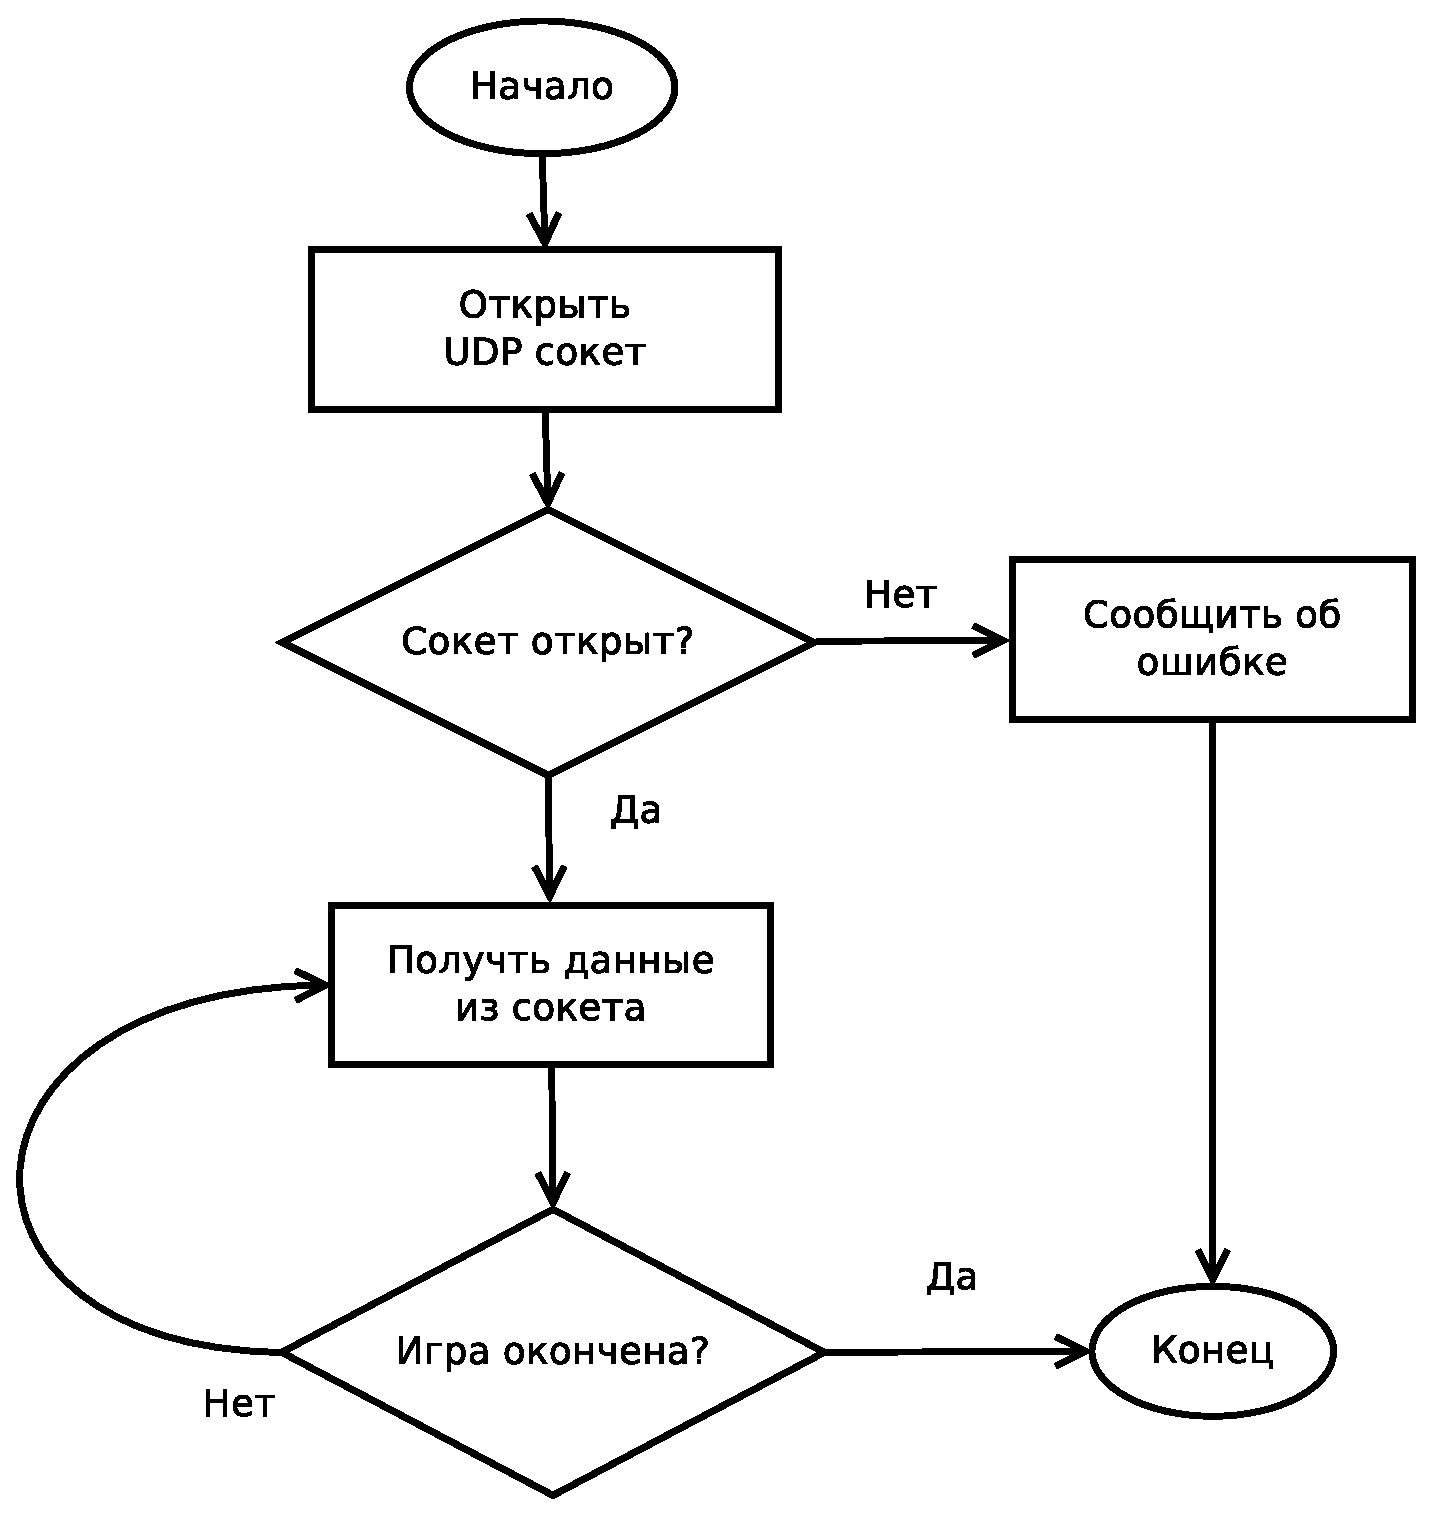
\includegraphics[width=0.5\linewidth]{2_3_2_gc}}
    \caption{Последовательность действий при взаимодействием с игровым контроллером}
    \label{im:2_3_2_gc}
\end{figure}

В данной реализации отсутствует класс нода из-за особенностей архитектуры. Каждый модуль можно описать группой методов, которые выполняются в определенном порядке и при определенных условиях. Данные методы можно обернуть в экземпляр функционального объекта и добавлять их в очередь задач при необходимости. Для примера можно взять модуль взаимодействия через сетевое соединение с игровым контроллером туртира RoboCup (рис. \ref{im:2_3_2_gc}): для взаимодействия используется UDP сокет, на который приходят данные о состоянии игры. В данном модуле можно выделить три метода, которые описывают все возможные действия: открыть UDP сокет, получить данные из сокета и сообщить об ошибке. Если сокет был успешно открыт, то в очередь задач добавляется функтор, отвечающий за получение данных из сокета, в противном случае в очередь задач добавляется функтор, отвечающий за обработку ошибки. По аналогии создаются функторы для других стадий алгоритма.

Такой подход к описанию модуля позволяет разбить его выполнение на множество небольших методов, которые зависят друг от друга, что в свою очередь уменьшает вероятность блокирование очереди задач одним модулем на длительный промежуток времени. При этом данный подход имеет два существенных недостатка: асинхронное приложение гораздо сложнее поддается отладке и требуется дополнительные расходы на аллокацию памяти под функторы и добавление в глобальную очередь задач, что может понизить производиетнльность всей системы при большом количестве задач.

В случае исполнения задач в пуле потоков отсутствует возможность обеспечить потокобезопасное исполнение модуля без блокировок и без дополнительных абстракций, которые существенно усложнили бы структуру всей системы. Из этого следует, что в данной реализации для потокобезопасного исполнения модулей без дополнительных примитивов внутри самих модулей разработчик должен гарантировать, что в очереди задач находится только одна задача одного модуля при условии, что система не будет обрабатывать функции обратного вызова при изменении состояния.

В асинхронной версии библиотеки существенно измененны механизмы синхронизации. В их основе все также лежат потокобезопасные очереди без блокировок с отложенными вызовами функций. В одном механизме может существовать несколько очередей синхронизации для упорядочивания асинхронных вызовов к механизму, например, сначала идет обработка запросов на изменение количества слушателей, после идет отправка сообщений на данные слушатели. В каждом механизме существует метод добавления в лаунчер задачи на применение изменений. Данный метод гарантирует, что задача на обновление добавлена в лаунчер только один раз, чтобы уменить потерю производительности, и все задачи будут выполнены в одном потоке.

Получение информации из системы так же осуществляется с использованием паттерна проектирования <<издатель-подписчик>>. Поскольку синхронизация может происходить параллельно с исполнением модулей, отсутствует возможность получить напрямую данные из системы, например, список слушателей. Для получения информации о существовании топика нужно зарегистрировать функтор для получения изменений о количестве топиков. При добавлении или удаления топика атоматически передается информация о событии всем слушателям.

Поскольку механизм использует функции обратного вызова существует вероятность, что эти функторы могут после выполнения добавлять в механизм новые задачи, что может привести к блокировки всей системы из-за того, что механизм будет работать бесконечно, постоянно добавляя себе новые задачи. Данная проблема решается ограничением количества вызовов за одну итерацию обработки входящих событий из очереди. Если во время исполнения был превышен лимит, то механизм повторно добавляет в очередь задачу обновления механизма.

На сегодняшний день существует асинхронная версия библиотеки для языка C++ с блокирующей синхронизацией, с помощью которой можно разработать подобную модульную систему - Boost Asio \cite{torjo2013boost}. Поскольку библиотека показывает достаточно высокие показатели производительности для асинхронной библиотеки, поддерживается большим сообществом разработчиков, то в рамках работы не планируется проектирование асинхронного фреймворка с блокирующей синхронизацией. В результатах тестирования быстродействия приведены сравнительные результаты производительности межмодульного взаимодействия и скорости исполнения очереди задач для асинхронного фреймворка с синхронизацией без блокировок и Boost Asio.






